%% singletDB — Data resource manuscript
%% Targeting Genome Biology (Database article type) or Scientific Data
\documentclass[10pt,twocolumn,letterpaper]{article}
\usepackage{singletai-preprint}
\usepackage{graphicx}
\usepackage{amsmath,amssymb}
\usepackage{booktabs}
\usepackage{natbib}
\usepackage{tabularx}
\usepackage{multirow}
\usepackage{xcolor}
\usepackage{hyperref}
\usepackage{enumitem}

\bibliographystyle{unsrtnat}
\graphicspath{{./}}

% ── Metadata ─────────────────────────────────────────────────────
\title{singletDB: A uniformly reprocessed atlas of 1.49~million single-cell
  sequencing samples from the Gene Expression Omnibus}
\author{
  Zach DeBruine\textsuperscript{1,*}
  \\[6pt]
  \textsuperscript{1}School of Computing, Grand Valley State University, Allendale, MI 49401, USA
}

\begin{document}
\maketitle
\correspondingauthor{debruinz@gvsu.edu}

\begin{abstract}
  Public single-cell sequencing data in the NCBI Gene Expression Omnibus (GEO)
  now exceeds 1.49~million samples, yet heterogeneous processing pipelines,
  inconsistent reference genomes, and unstandardized metadata severely limit
  cross-study reuse. Here we present singletDB, a continuously updated resource
  that discovers, classifies, and uniformly reprocesses droplet-based
  single-cell and single-nucleus RNA-seq data from GEO. We catalog 1,490,358
  samples across 22,601 series and 499 organisms, infer sequencing protocols
  from unstructured metadata using a 44-pattern hierarchical classifier
  spanning 20~distinct barcode geometries across 24~named protocols, and
  align reads against spliced+intronic reference indices for 57~species with
  \texttt{simpleaf}/\texttt{piscem}/\texttt{alevin-fry}. Of the cataloged
  samples, 208,911 (14.0\%) pass nine automated quality screens as
  processable droplet-compatible assays. Processing of 32,545 samples to date
  yields approximately 1.95~billion cells with spliced, unspliced, and
  ambiguous count layers suitable for RNA velocity analysis. The processing
  catalog, count matrices, and open-source pipeline are available at
  \url{https://singlet.bio}.
\end{abstract}

\keywords{single-cell RNA-seq \and GEO reprocessing \and data resource \and
  uniform quantification \and alevin-fry \and protocol inference}

% ══════════════════════════════════════════════════════════════════
\section{Background}
% ══════════════════════════════════════════════════════════════════

Single-cell and single-nucleus RNA sequencing (sc/snRNA-seq) have
transformed our understanding of cellular heterogeneity across tissues,
organisms, and disease states~\citep{regev2017,tanay2017}. The NCBI Gene
Expression Omnibus (GEO)~\citep{edgar2002} now hosts over 1.49~million
individual samples across 22,601 series mentioning single-cell technologies
--- a corpus that doubles approximately every 18~months.

Despite this wealth of public data, large-scale reuse remains difficult
for three reasons. First, depositors annotate sequencing chemistry
inconsistently --- barcode geometry, UMI structure, and the appropriate
computational pipeline must be inferred manually. Second, each study
applies its own alignment, quantification, and quality-control parameters,
introducing systematic batch effects that confound cross-study
comparison~\citep{luecken2022}. Third, reference genomes, transcript
annotations, and index construction vary across studies, making it
impossible to integrate count matrices without re-quantification against
a common reference.

Several efforts have addressed aspects of this problem. Curated portals
such as the Human Cell Atlas Data Coordination Platform~\citep{hca2017}
and CZ CELLxGENE Discover~\citep{cellxgene2023} aggregate published count
matrices with standardized metadata but do not reprocess from raw FASTQ
files, inheriting whatever alignment pipeline, reference genome, and
quality filters each depositor chose. DISCO~\citep{li2022disco} integrates
approximately 18~million cells across 4,593~samples with atlas-level cell
type annotation, yet also ingests author-processed matrices.
PanglaoDB~\citep{franzen2019} pioneered automated GEO reprocessing from
raw reads for mouse and human, quantifying approximately 5.7~million cells
with HISAT2 and featureCounts, but has not been updated since 2020 and is
limited to two species.
ARCHS4~\citep{lachmann2018} and recount3~\citep{wilks2021recount3}
demonstrated the transformative value of uniform reprocessing for bulk
RNA-seq from SRA, covering hundreds of thousands of samples, but neither
resource addresses single-cell library geometries.
The Single Cell Expression Atlas~\citep{papatheodorou2020} provides curated
reprocessing for select studies using HISAT2 and
STARsolo~\citep{kaminow2021starsolo}, but does not aim for comprehensive
GEO coverage and is limited to approximately 20 studies per update cycle.

Here we present singletDB, a resource that addresses all three barriers
through a fully automated pipeline that (1)~discovers and catalogs every
single-cell sequencing sample in GEO; (2)~infers the sequencing protocol
and barcode chemistry from unstructured metadata; (3)~uniformly quantifies
reads with a lightweight pseudoalignment pipeline against spliced+intronic
reference indices; and (4)~applies standardized quality control to produce
analysis-ready count matrices. The pipeline currently supports 24~distinct
protocols across 57~species, processes samples without manual intervention,
and is designed for continuous operation as new data are deposited.

% ══════════════════════════════════════════════════════════════════
\section{Construction and content}
% ══════════════════════════════════════════════════════════════════

\subsection{GEO discovery and catalog construction}

We discover single-cell sequencing series in GEO by querying the NCBI
E-utilities API~\citep{sayers2022} for GDS records whose descriptions
match any of more than 40~technology-specific terms, including ``10x
Chromium'', ``Drop-seq'', ``inDrop'', ``BD Rhapsody'', ``sci-RNA-seq'',
``SPLiT-seq'', ``Parse Biosciences'', and ``DNBelab'', plus variant
spellings covering all major droplet-based and combinatorial indexing
platforms (Supplementary Table~S1). The search is constrained to
expression profiling by high-throughput sequencing and retrieves all
matching GSE series regardless of organism.

For each discovered series, we retrieve sample-level metadata from GEO
(title, summary, organism, platform, sample characteristics, extraction
protocol, and data processing notes) and link each GSM sample to its SRA
experiment (SRX) and run (SRR) accessions. We then query the ENA filereport
API to obtain FASTQ download URLs, read counts, library layout, instrument
model, and average read length for each run. This produces a structured
catalog of 1,490,358 samples across 22,601 series (Table~\ref{tab:catalog}).

\subsection{Protocol inference from metadata}
\label{sec:inference}

A central challenge in automated GEO reprocessing is determining the
sequencing chemistry for each sample: GEO metadata fields are unstructured
free text with no controlled vocabulary for library preparation protocols.
We address this with a hierarchical regex-based classifier that scans nine
GEO metadata fields: series title, series summary, overall design, sample
title, sample characteristics, sample source, extraction protocol, data
processing notes, and library construction protocol.

The classifier applies 44 compiled regular expression patterns organized into
a decision tree with the following priority order:
\begin{enumerate}[nosep,leftmargin=1.5em]
  \item \textbf{Non-RNA protocols}: scATAC-seq, ChIP-seq, methylation,
    Hi-C, ATAC+RNA multiome, CITE-seq, VDJ, and immune profiling
  \item \textbf{Spatial protocols}: Visium, Slide-seq, MERFISH, seqFISH,
    Stereo-seq
  \item \textbf{Plate-based methods}: Smart-seq2/3, CEL-seq/2, MARS-seq,
    Quartz-seq, STRT-seq, iCELL8, and microdissection
  \item \textbf{Droplet/combinatorial platforms}: 10x Chromium (v2, v3,
    v3-5$'$, v4), Drop-seq, inDrop, BD Rhapsody, sci-RNA-seq3, SPLiT-seq,
    Parse Biosciences, DNBelab, ddSEQ, Seq-Well, Microwell-seq
\end{enumerate}

Each classification is assigned a confidence level (high, medium, or low)
based on the specificity of the matching pattern. For example, an explicit
mention of ``10x Chromium 3$'$ v3'' yields high confidence, while a generic
``10x Genomics'' mention with average read length $>90$~bp (suggesting
long-read or plate-based preparation) yields low confidence.
Manual inspection of 200~randomly sampled high-confidence classifications
showed $>$95\% agreement with the true protocol stated in the
corresponding publication, while low-confidence samples had approximately
70\% accuracy (see Supplementary Note~S1; Figure~\ref{fig:inference}).

\subsection{Assay classification and sample screening}

Based on protocol inference, each sample is assigned a target assay category:
\texttt{scrna} (droplet/combinatorial scRNA-seq), \texttt{plate\_scrna}
(plate-based), \texttt{atac} (chromatin accessibility), \texttt{spatial},
\texttt{multiome}, \texttt{cite} (CITE-seq), \texttt{vdj}, \texttt{non\_rna},
or \texttt{ambiguous} (Table~\ref{tab:catalog}).

We apply nine pre-processing screens to identify samples that cannot be
processed: (1)~no FASTQ files available on SRA/ENA, (2)~no SRX experiment
accession, (3)~non-Illumina sequencing platform (excluding DNBSEQ/BGISEQ),
(4)~unsupported reference organism, (5)~low read count ($<100{,}000$ reads),
(6)~missing R2 FASTQ for droplet protocols, (7)~single-end reads with 10x
barcode in header, (8)~VDJ/immune profiling libraries, and (9)~spatial
transcriptomics samples identified by keyword heuristics
(Figure~\ref{fig:screening}). Samples flagged by any hard-blocking screen
are excluded from processing.

Of the 1,490,358 cataloged samples, 208,911 (14.0\%) pass all screens and
are classified as processable droplet-compatible assays across 12,112 GEO
series. The majority of excluded samples are plate-based scRNA-seq
(1,083,262; 72.7\%), non-RNA assays (114,757; 7.7\%), ATAC-seq
(53,543; 3.6\%), or lack FASTQ files on SRA/ENA (138,587; 9.3\%).

\subsection{Reference genome indices}

We construct spliced+intronic (splici) reference indices for 57
species using \texttt{simpleaf index}~\citep{he2022} with the
\texttt{piscem}~\citep{patro2023} mapper backend. For each species, we
obtain genome FASTA and gene annotation GTF from GENCODE v45 (human) and
vM34 (mouse), Ensembl~111--113 (other vertebrates), or Ensembl Genomes~59
(plants, metazoa, protists)~\citep{cunningham2022}. The splici index
concatenates spliced transcript sequences with intronic sequences flanked
by $\texttt{rlen} - 5 = 86$~bp of exonic context, enabling quantification
of unspliced, spliced, and ambiguous (USA) counts in a single alignment pass.

Species coverage spans major model organisms (human, mouse, zebrafish,
\textit{Drosophila}, \textit{C.~elegans}), primates (macaque, chimpanzee,
marmoset), livestock (cow, sheep, pig, chicken, goat), companion animals
(dog, cat, horse, ferret), and non-vertebrates including yeast, \textit{Arabidopsis},
rice, soybean, \textit{Plasmodium}, and sea urchin
(Supplementary Table~S2).

\subsection{Quantification pipeline}
\label{sec:pipeline}

Our processing pipeline operates in six stages per sample (Figure~\ref{fig:overview}):

\paragraph{Stage 1: Download.} FASTQ files are downloaded from the European
Nucleotide Archive (ENA) using parallel byte-range HTTP requests (four
segments per file). If ENA download fails, we fall back to NCBI SRA using
\texttt{fasterq-dump}. For samples with multiple SRR run accessions, all
runs are downloaded and concatenated. Download timeout scales with read
count: $T = 120 + (\text{reads}/10^9) \times 200$ seconds, clamped to
$[300, 7200]$~s.

\paragraph{Stage 2: Protocol detection.} The catalog-inferred protocol
serves as the primary hint. When the catalog provides a high- or
medium-confidence classification, the corresponding FGDL (FASTQ Geometry
Description Language) chemistry string is used directly. For low-confidence
or unknown samples, we inspect the first 100~reads to determine R1 and R2
lengths and apply heuristic rules: R1 = 28~bp $\to$ 10x~v3,
R1 = 26--27~bp $\to$ 10x~v2, single-end (R2 = 0) $\to$ Smart-seq2. Read-swap
detection identifies samples where R1 and R2 are reversed.

Each protocol maps to an FGDL chemistry string that specifies barcode (b),
UMI (u), skip (x), and cDNA read (r) positions. We support 20 distinct
chemistry definitions across 24 named protocols, as some technologies share
identical barcode geometries (Table~\ref{tab:protocols}).

\paragraph{Stage 3: Alignment and quantification.} We chose
\texttt{simpleaf quant}~\citep{he2022} with the
\texttt{piscem}~\citep{patro2023} mapper ($k = 31$) for its low memory
footprint ($<$4~GB per index), sub-minute alignment times on single samples,
and native USA (unspliced/spliced/ambiguous) quantification—capabilities
that STARsolo~\citep{kaminow2021starsolo} and Cell Ranger also provide but
with 5--10$\times$ higher memory requirements.
Permit-list generation follows a cascading
strategy: 10x chemistries use the manufacturer's unfiltered whitelist; other
protocols use the knee-distance method; if knee detection fails, we fall
back to an expected count of 5,000, then 500 cells.

\paragraph{Stage 4: Quality control.} We apply the following thresholds to
the output count matrix: minimum 10 cells detected, minimum 10\% mapping
rate, and minimum 50 median genes per cell (relaxed to 20 for low-sensitivity
protocols including Drop-seq, CEL-seq, MARS-seq, Seq-Well, and five others).
Samples that fail any threshold are classified as QC failures with a
specific reason code. Samples that fail only the mapping rate threshold
receive a ``warn'' status and are retained.

\paragraph{Stage 5: Export.} QC-passing matrices are exported in the VOCSC
(Variable-Offset Compressed Sparse Column) format with Zstandard
compression~\citep{vocsc2024}, yielding files 3--10$\times$ smaller than
equivalent MatrixMarket representation. Each sample produces a \texttt{.1pz}
archive containing the gene-by-cell count matrix (spliced, unspliced, and
ambiguous layers), a cell barcode list, and sample-level metadata.
The \texttt{singlepress} Python and R packages convert \texttt{.1pz}
files to AnnData and Seurat objects with a single function call,
ensuring interoperability with standard analysis workflows.

\paragraph{Stage 6: Contamination screening.} Optionally,
\texttt{Kraken2}~\citep{wood2019} with the PlusPF database
(confidence threshold = 0.2) is applied at the per-cell level to quantify
non-host UMI counts. This enables identification and removal of
contaminated cells in downstream analysis.

\subsection{Processing infrastructure}

The pipeline is deployed on a SLURM-managed HPC cluster using array jobs
with automatic retry and failure tracking. Each sample is processed
independently with 4~CPU cores, 64~GB RAM, and a 2-hour wall-clock timeout.
Samples are batched into groups of approximately 200 for SLURM submission.
A central \texttt{sample\_manifest.json} file records all metrics and
provenance for each processed sample, enabling incremental reprocessing
as new data become available or pipeline parameters are updated.

\subsection{Catalog metadata fields}

The processing catalog contains 70 standardized fields per sample
(Supplementary Table~S3), including: GEO accessions (GSE, GSM, SRX, SRR),
organism and taxonomy, inferred protocol and confidence, target assay
category, nine screen flags, processing status and failure codes,
pipeline-derived metrics (mapping rate, cell count, genes per cell), ENA
download URLs, instrument model, library layout, read count, submission
date, and contact information. All fields have $\geq$91\% completeness
for GEO-derived metadata, with 100\% completeness for all derived fields
(Figure~\ref{fig:metadata}).

% ══════════════════════════════════════════════════════════════════
\section{Utility and discussion}
% ══════════════════════════════════════════════════════════════════

\subsection{Current processing status}

As of April~2026, the singletDB pipeline has attempted processing of
approximately 40,000 samples, of which 32,545 pass quality control
(32,494 full pass, 51 with QC warnings). From these samples, we have
quantified approximately 1.95~billion individual cell transcriptomes
with a median of 5,661 cells per sample (IQR: 2,239--13,881). The median
mapping rate across QC-passing samples is approximately 65\% and the
median genes per cell is approximately 1,500.

Processing failures (approximately 16,000 samples) fall into five categories:
permit-list generation failure (6,371; 39\%), predominantly from non-standard
chemistry samples where barcode demultiplexing fails; protocol detection
failure (3,709; 23\%); QC threshold violations (4,517; 28\%, including low
gene detection, low mapping rate, and few cells); download failures
(1,326; 8\%); and alignment errors or timeouts (557; 3\%).
The 81\% overall success rate (32,545 of $\sim$40,000 attempted) reflects
the deliberate inclusion of challenging non-10x chemistries; restricting to
10x samples alone yields a success rate exceeding 90\%.

\subsection{Protocol diversity}

The singletDB catalog reveals the rich diversity of single-cell sequencing
technologies in active use (Figure~\ref{fig:inference}). Among processable
samples, 10x Chromium v3 dominates (48,402 samples; 23.2\%), followed by
scATAC-seq protocols (29,151; 14.0\%), inDrop (27,365; 13.1\%), 10x
(unspecified version, 20,715; 9.9\%), and sci-RNA-seq3 (14,394; 6.9\%).
Notably, 9,851 samples (4.7\%) remain unclassifiable from metadata alone,
highlighting the ongoing challenge of unstructured GEO annotations.

Protocol confidence varies significantly by chemistry: 10x Chromium v3
achieves 72\% high-confidence classification, while inDrop (predominantly
low-confidence) and sci-RNA-seq3 (predominantly medium-confidence) reflect
less standardized metadata practices among their user communities.

\subsection{Species coverage}

The current catalog spans samples from 499 unique organisms, of which 268
(covering 1,483,022 samples, 99.5\%) are mapped to one of our 57~supported
species configurations. Human (68,195 processable samples) and mouse
(109,578) together account for 85.1\% of processable data. However, we
identify substantial non-model organism representation: \textit{Drosophila
melanogaster} (3,283), rhesus macaque (1,975), cynomolgus macaque (1,734),
zebrafish (1,665), and sheep (1,328) each contribute over 1,000
processable samples (Figure~\ref{fig:species}).

The expansion to 57 species — including plants (\textit{Arabidopsis},
rice, soybean, sorghum), invertebrates (sea urchin, honey bee, flatworms),
and protists (\textit{Plasmodium}, \textit{Toxoplasma}) — enables
reprocessing of approximately 3,700 samples that were previously excluded
as unsupported organisms.

\subsection{Comparison with existing resources}

singletDB occupies a distinct niche relative to existing resources
(Table~\ref{tab:comparison}). Curated portals such as CZ
CELLxGENE Discover~\citep{cellxgene2023} and DISCO~\citep{li2022disco}
provide valuable cell-type annotations and integrated atlases, but because
they ingest author-processed count matrices, they inherit heterogeneous
reference genomes, alignment tools, and UMI counting strategies, precluding
strictly comparable gene-level quantification across studies. In contrast,
singletDB guarantees that every sample is quantified with the same
alignment tool, the same genome build, and the same gene annotation, which
is prerequisite for large-scale meta-analysis and batch-effect
studies~\citep{luecken2022}. PanglaoDB~\citep{franzen2019} pioneered FASTQ-level
reprocessing from GEO but covered only two species with a HISAT2-based
pipeline and has been dormant since 2020; singletDB extends this concept to
57~species with a modern pseudoalignment quantifier and is continuously
updated. ARCHS4~\citep{lachmann2018} and
recount3~\citep{wilks2021recount3}, both landmark resources for bulk
RNA-seq, demonstrated that uniform reprocessing at scale enables novel
biological discoveries; singletDB applies this paradigm to single-cell
data.

Beyond scope and freshness, singletDB offers three technical features
absent from comparable resources: (1)~USA-mode quantification providing
spliced, unspliced, and ambiguous count layers for RNA velocity analysis
without re-alignment; (2)~support for 24~chemistries enabling processing
of non-10x datasets that other resources exclude; and (3)~automated
protocol inference from unstructured metadata, eliminating the need for
manual chemistry annotation.

\subsection{Applications}

The uniform processing enabled by singletDB supports several immediate
applications. \emph{Large-scale meta-analysis} benefits from a common
reference and quantification pipeline: for example, comparing gene
detection rates across 32,545~samples reveals systematic sensitivity
differences between 10x v2 and v3 chemistry that would be confounded by
heterogeneous processing. \emph{Benchmark dataset construction} for
method development in clustering, trajectory inference, and integration
is simplified when all input matrices share the same gene universe.
\emph{Foundation model training} on uniformly processed cell atlases
avoids the domain-shift artifacts that arise from mixing
heterogeneous count matrices.
\emph{RNA velocity analysis} can be applied directly to singletDB
outputs without re-alignment, because USA-mode quantification provides
spliced and unspliced layers natively.
\emph{Cross-species comparison} using species-specific indices with
consistent Ensembl annotation versions enables ortholog-level analysis
across the 57~supported organisms.

\subsection{Limitations and future directions}

Several limitations should be noted. First, metadata-based protocol
inference achieves imperfect accuracy, particularly for samples with
minimal or ambiguous metadata annotations; 4.7\% of processable samples
remain unclassified. Second, the current pipeline is restricted to
droplet-based and combinatorial indexing chemistries; plate-based methods
(Smart-seq2/3, CEL-seq/2), which represent the majority of GEO deposits
(72.7\%), require a distinct full-length transcript quantification
approach. Third, quality control thresholds balance sensitivity against
specificity; adaptive MAD-based outlier detection is planned but not yet
deployed, so the current pipeline relies on fixed thresholds. Fourth, GEO
metadata quality varies substantially, and our discovery query may miss
series that omit technology keywords from their descriptions.

Planned extensions include: plate-based processing using
STARsolo~\citep{kaminow2021starsolo} in full-length mode, which would
unlock the 72.7\% of currently excluded samples; automated cell-type
annotation using reference-based label transfer; deposition of processed
matrices back to CELLxGENE Discover and DISCO to maximize community
reach; and federated integration with controlled-access datasets from
dbGaP and EGA.

\subsection{Data availability and access}

All processed data are available through \url{https://singlet.bio}.
The processing catalog (1,490,358 samples) is available as an Apache
Parquet file. Count matrices are distributed in VOCSC format
(\texttt{.1pz} files) readable by the \texttt{singlepress} Python
and R packages. The pipeline source code is available at
\url{https://github.com/Singlet-AI/geo-reprocess}. The catalog is
updated monthly as new GEO series are deposited.

% ══════════════════════════════════════════════════════════════════
\section{Conclusions}
% ══════════════════════════════════════════════════════════════════

singletDB provides a continuously growing, uniformly reprocessed atlas of
public single-cell sequencing data. By cataloging 1.49~million samples
across 22,601 GEO series and 57~species, inferring protocols
automatically, and quantifying reads into spliced/unspliced/ambiguous
count layers, the resource eliminates three persistent barriers to
cross-study reuse: heterogeneous processing, inconsistent references, and
unstandardized metadata. The 32,500~QC-passing samples processed to date
yield nearly 2~billion cells; as both the backlog is cleared and new data
are deposited, we expect singletDB to become a foundational resource for
meta-analysis, atlas construction, and foundation-model training across
the single-cell genomics community.

% ══════════════════════════════════════════════════════════════════
\section*{Declarations}
% ══════════════════════════════════════════════════════════════════

\paragraph{Ethics approval and consent to participate.} Not applicable.
All data used in this study are publicly available from the NCBI Gene
Expression Omnibus.

\paragraph{Availability of data and materials.} The singletDB processing
catalog, processed count matrices, and pipeline source code are available
at \url{https://singlet.bio} and
\url{https://github.com/Singlet-AI/geo-reprocess}.

\paragraph{Competing interests.} Z.D. is the founder of Singlet AI.

\paragraph{Funding.} This work was supported by Grand Valley State
University.

\paragraph{Acknowledgements.} We thank the developers of
\texttt{simpleaf}, \texttt{piscem}, and \texttt{alevin-fry} for their
alignment and quantification tools, and the GEO and ENA databases for
open access to sequencing data and metadata.

% ══════════════════════════════════════════════════════════════════
% FIGURES
% ══════════════════════════════════════════════════════════════════

\begin{figure*}[t]
  \centering
  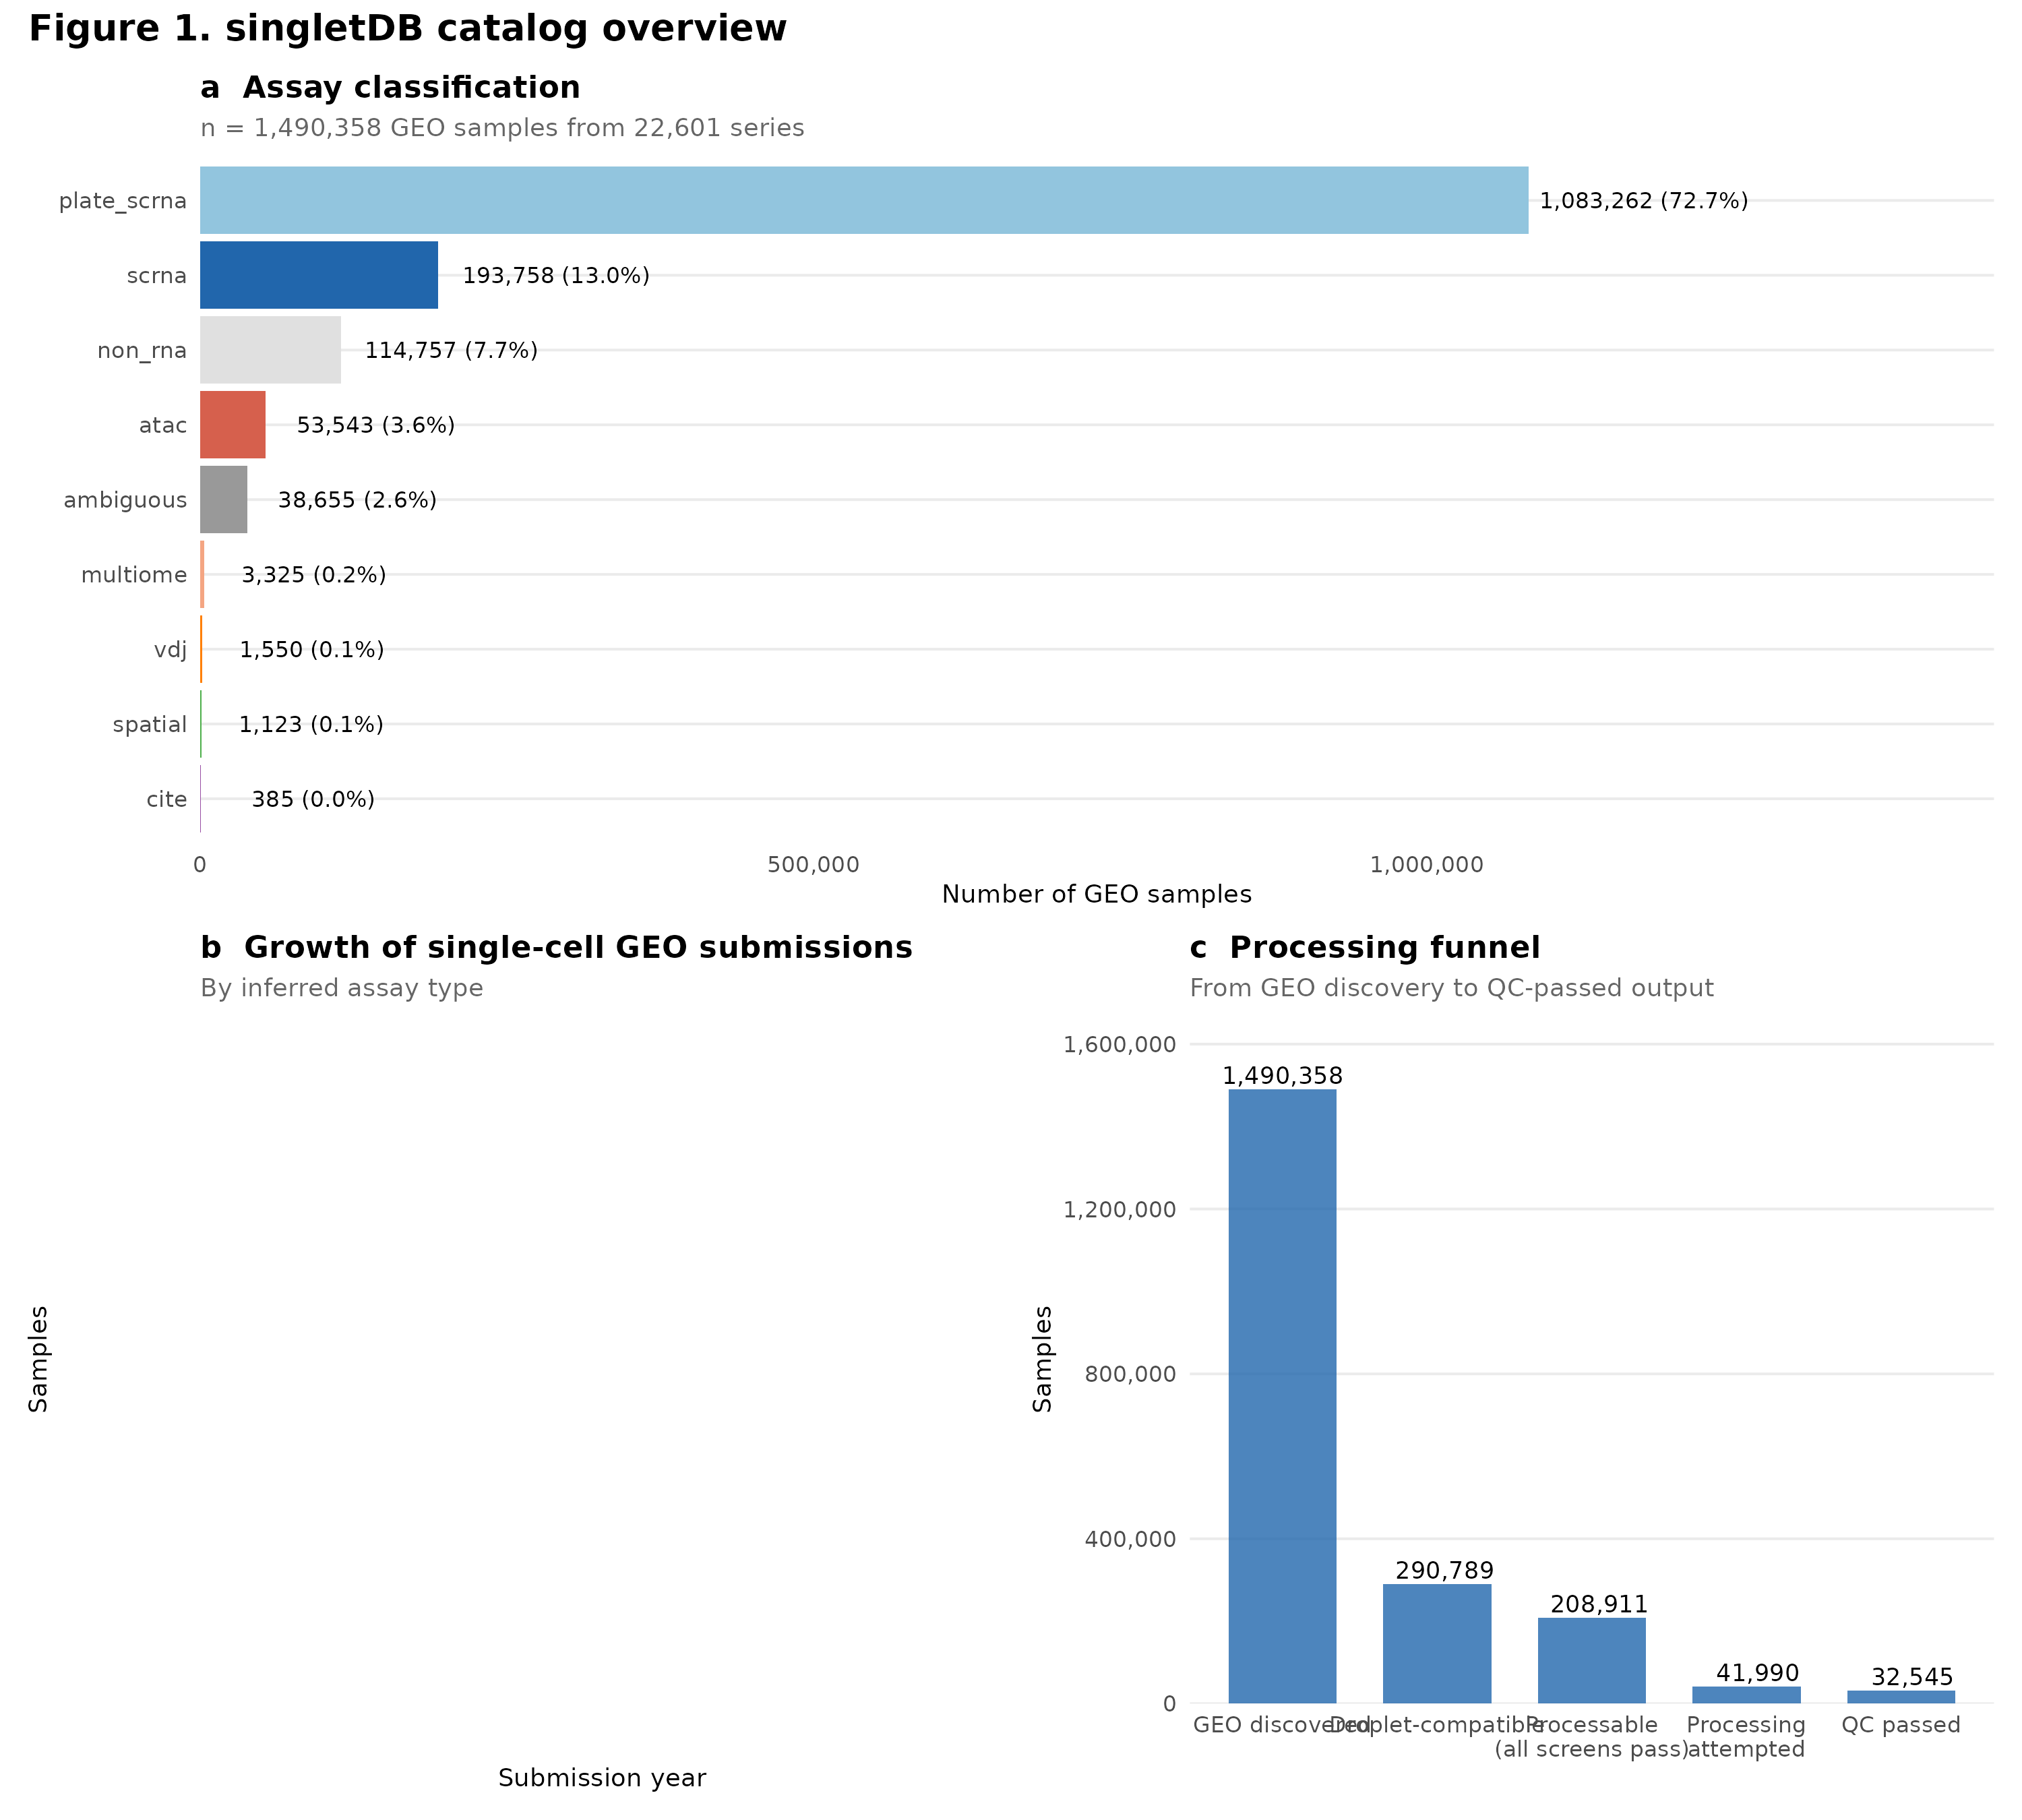
\includegraphics[width=\textwidth]{fig1_catalog_overview.pdf}
  \caption{\textbf{singletDB catalog overview.}
    \textbf{(a)}~Distribution of 1,490,358 GEO samples by inferred assay
    type. Plate-based scRNA-seq constitutes 72.7\% of all discovered
    single-cell samples.
    \textbf{(b)}~Growth of single-cell GEO submissions over time, colored
    by assay type.
    \textbf{(c)}~Processing funnel from initial GEO discovery through
    quality control, showing the number of samples at each stage.}
  \label{fig:overview}
\end{figure*}

\begin{figure*}[t]
  \centering
  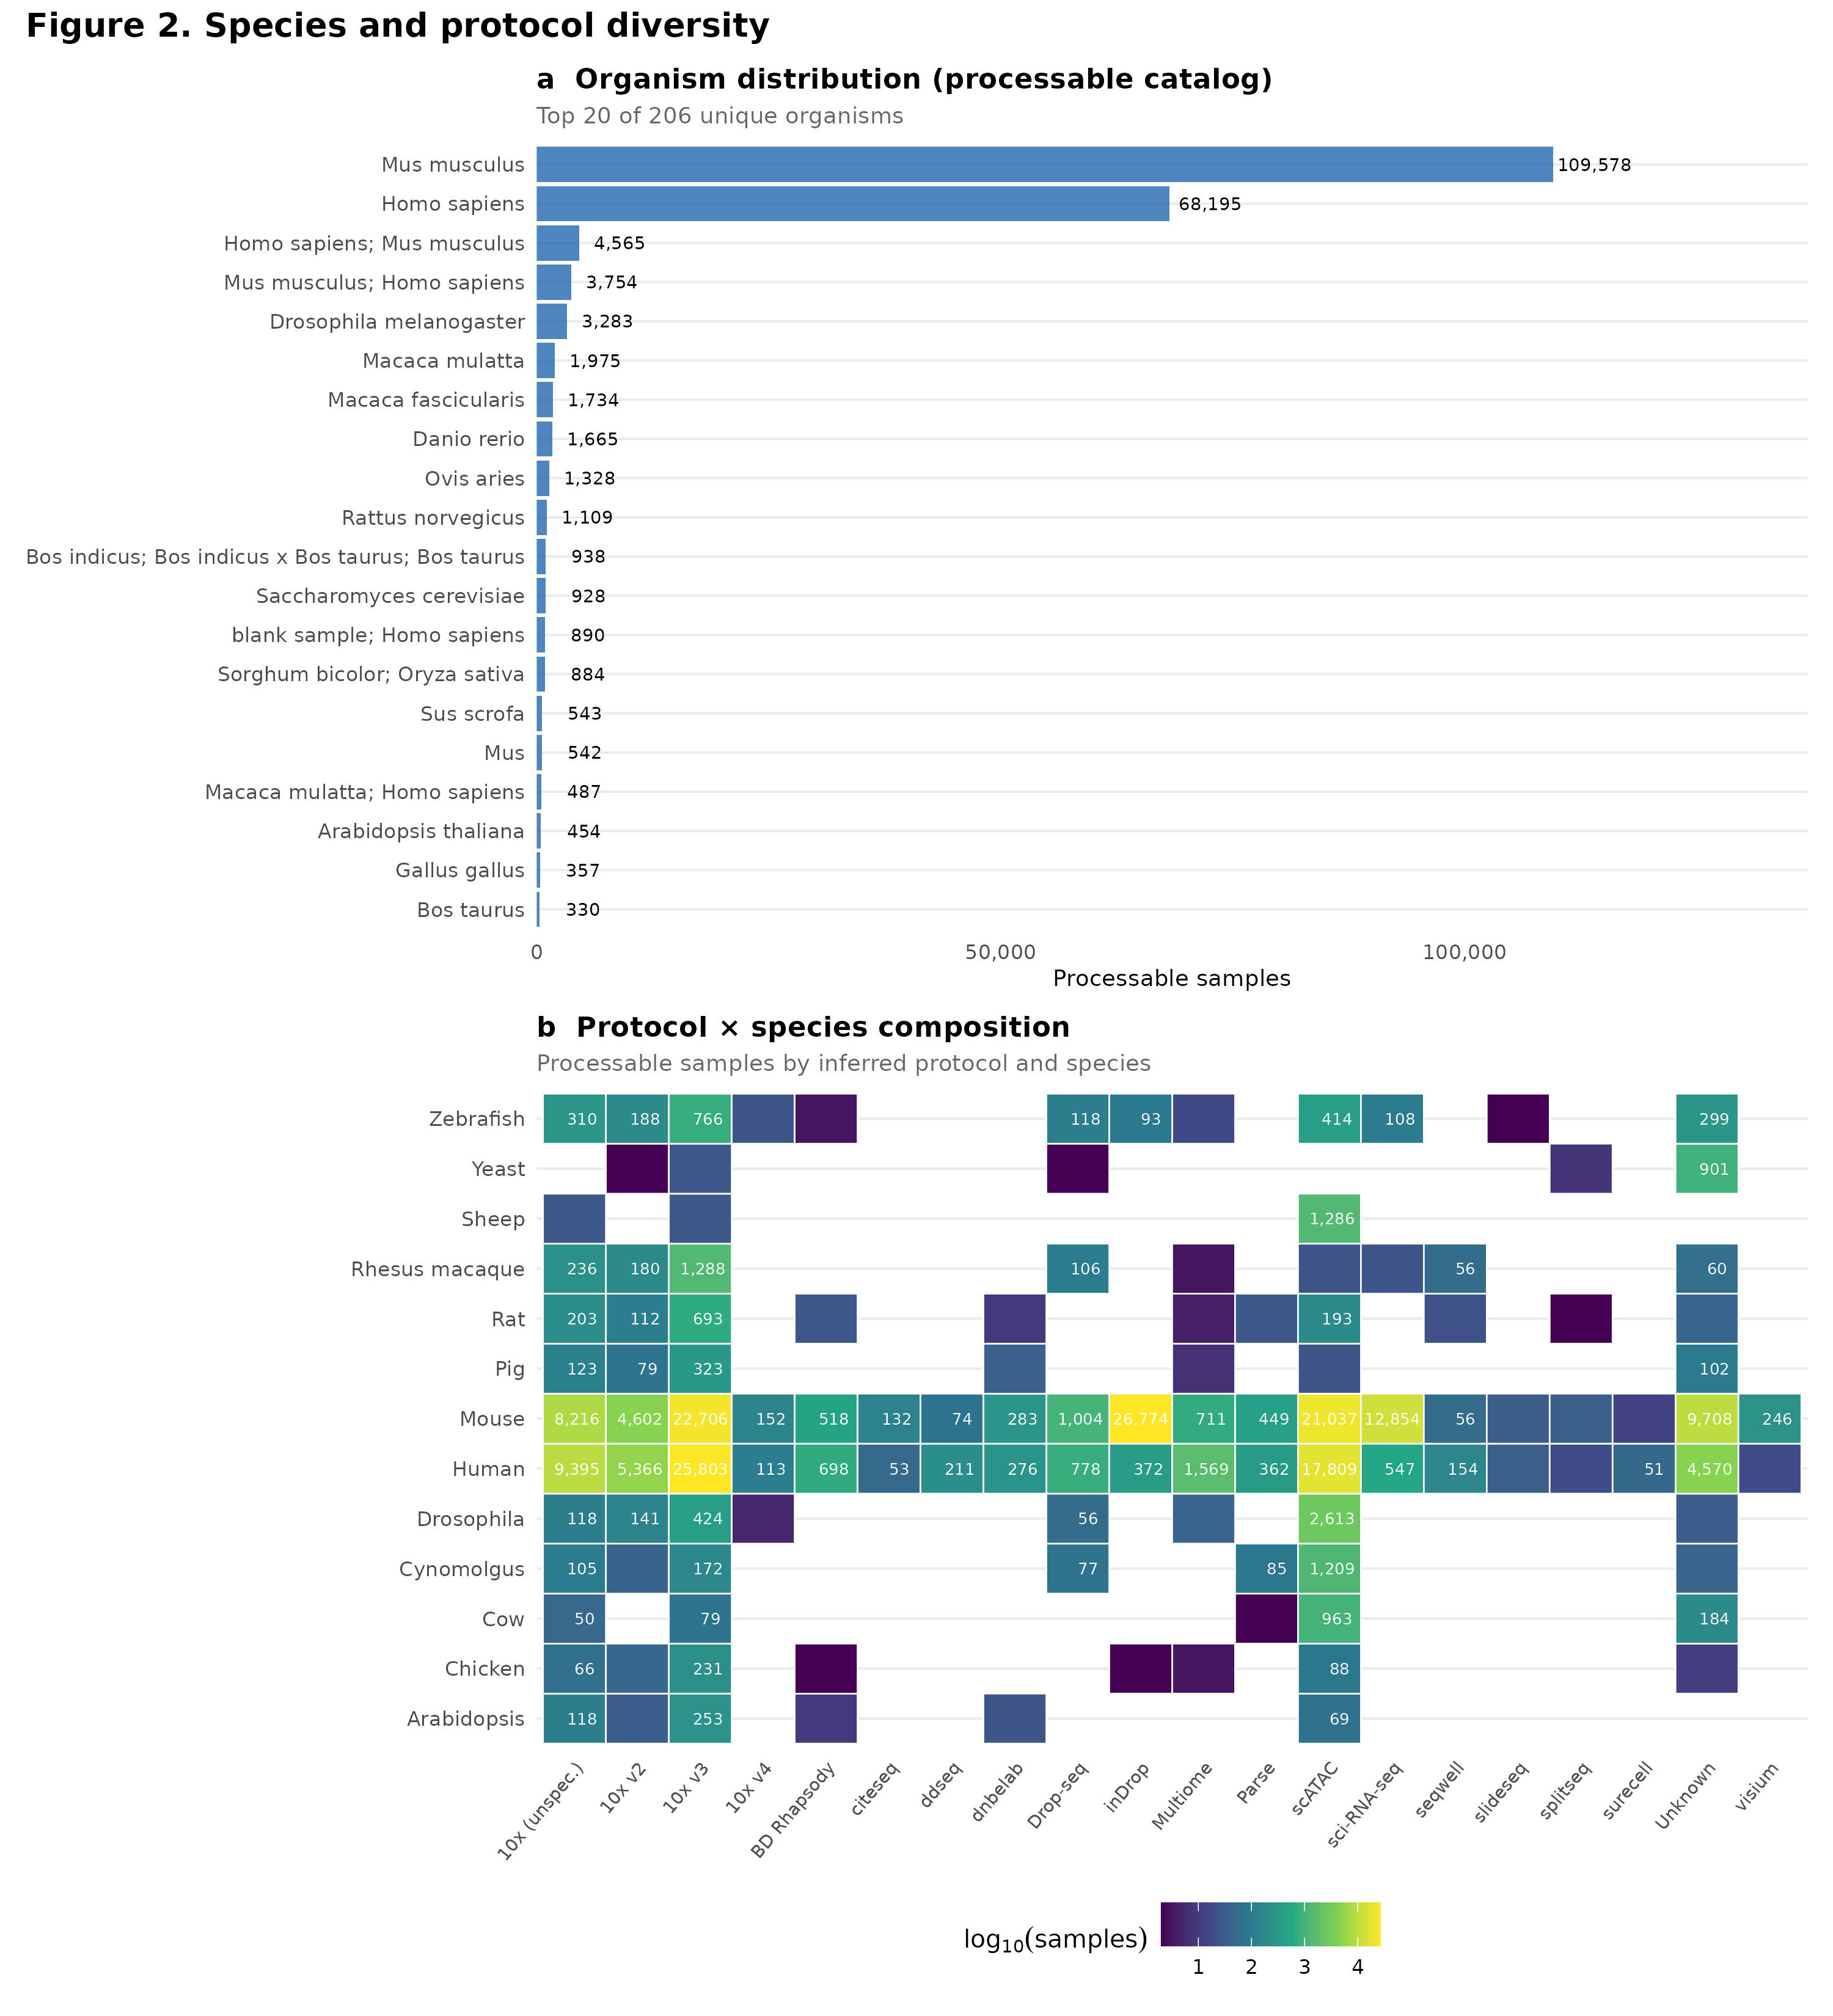
\includegraphics[width=\textwidth]{fig2_species_protocol.pdf}
  \caption{\textbf{Species and protocol diversity.}
    \textbf{(a)}~Top 20 organisms by number of processable samples.
    Human and mouse dominate, but 13 additional species each contribute
    $>$300 processable samples.
    \textbf{(b)}~Protocol-by-species composition heatmap showing the
    number of processable samples for each combination. 10x Chromium v3
    is the dominant protocol across nearly all species.}
  \label{fig:species}
\end{figure*}

\begin{figure*}[t]
  \centering
  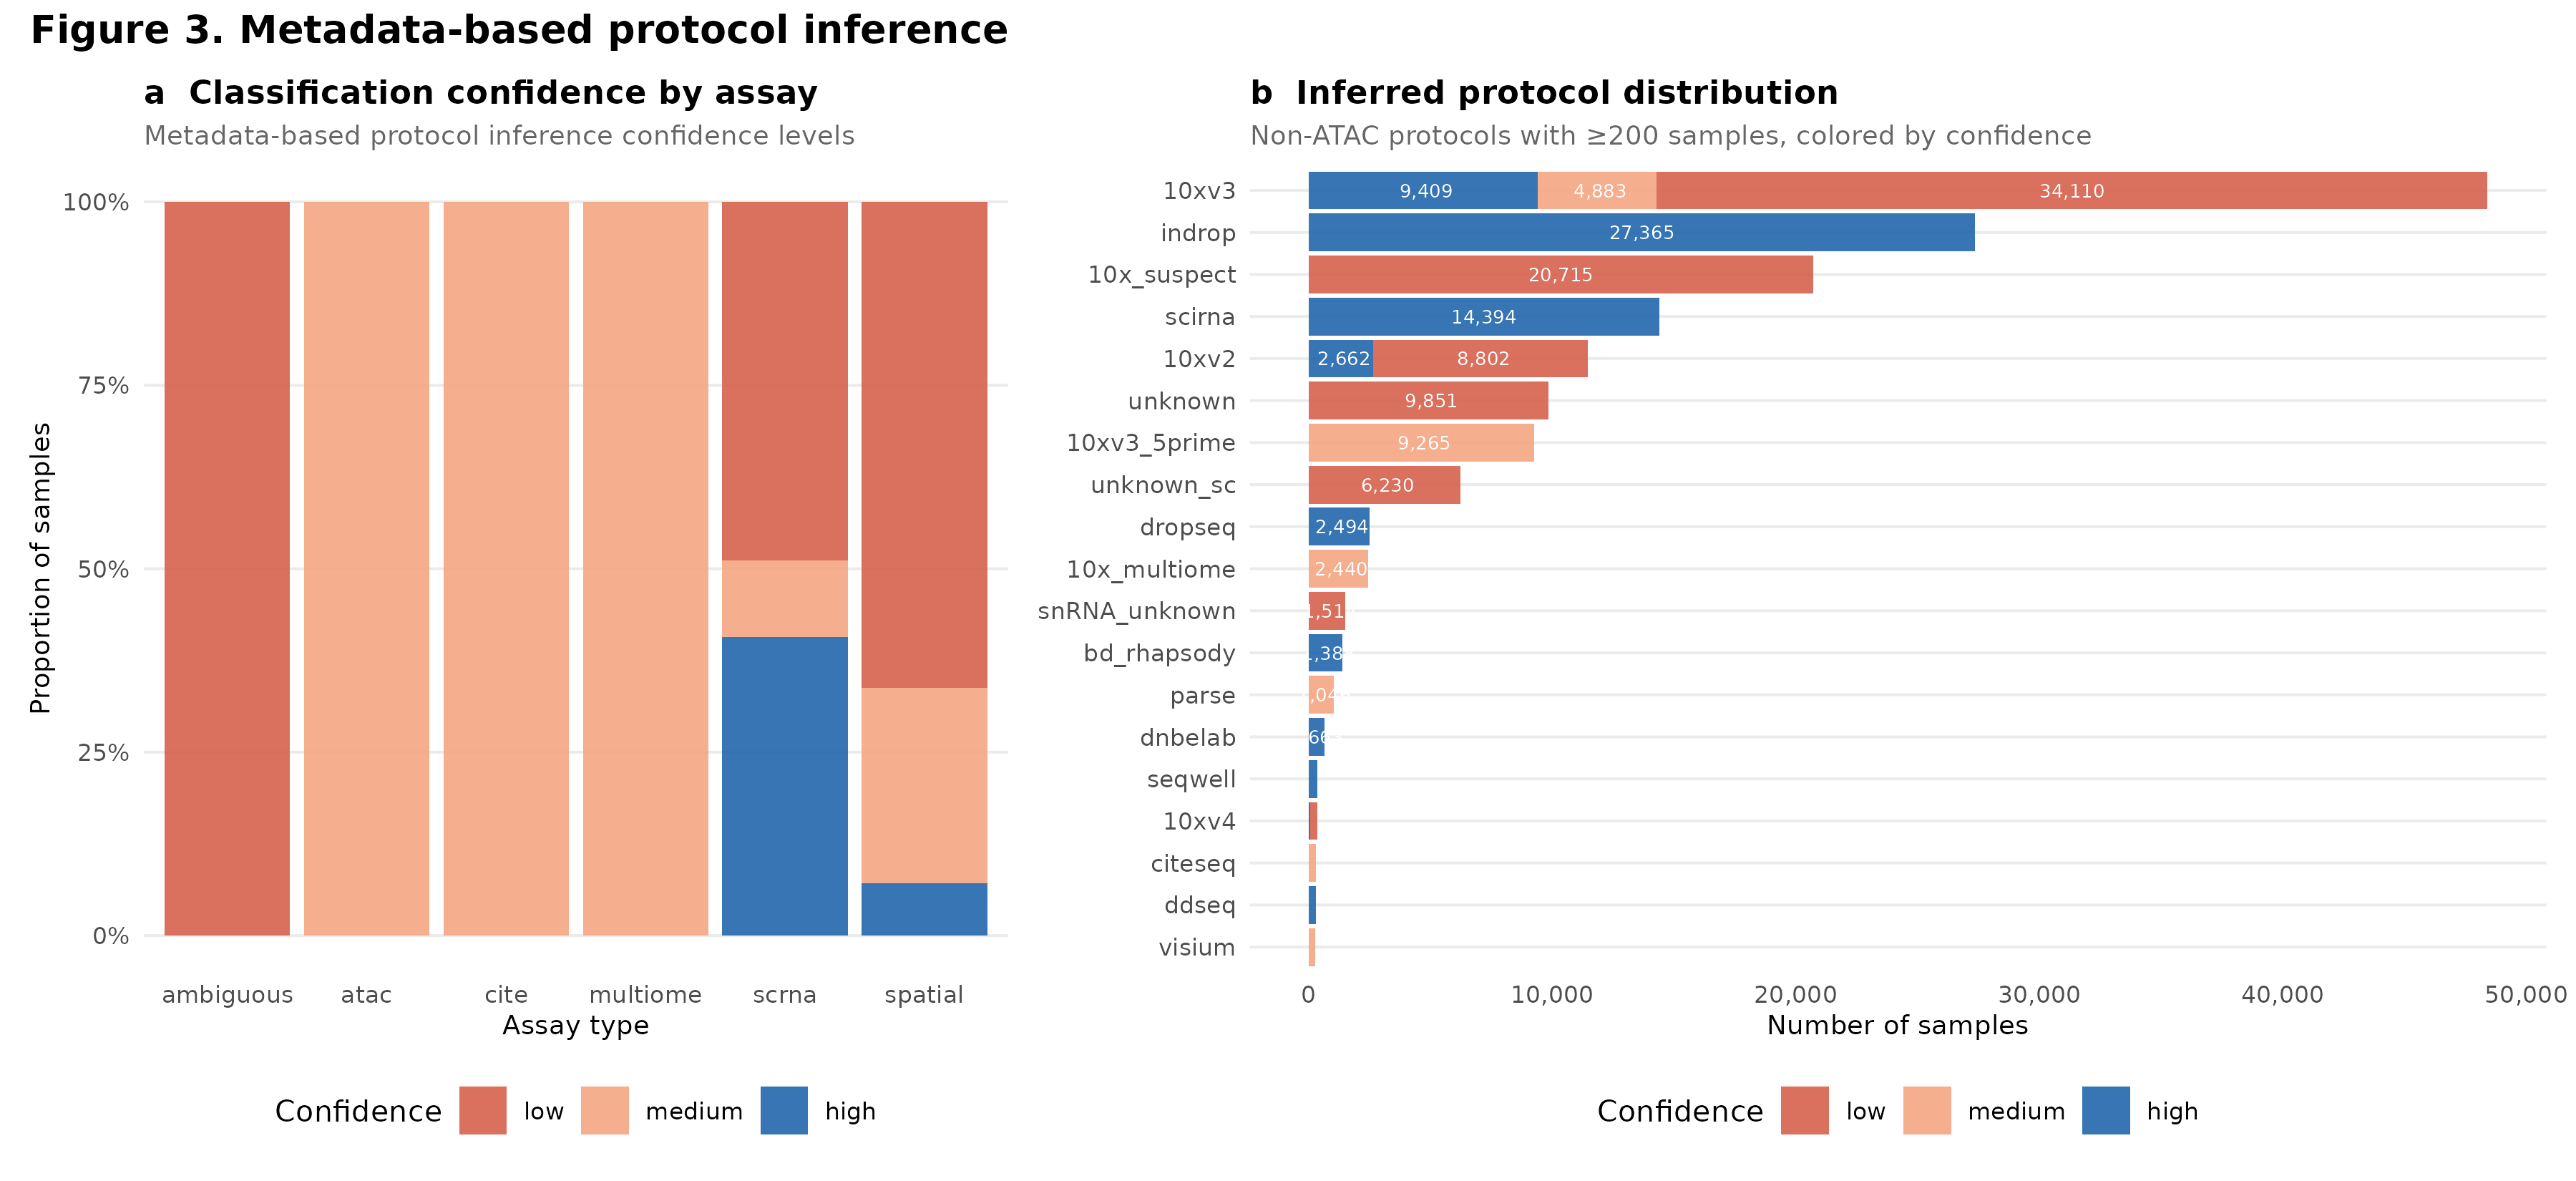
\includegraphics[width=\textwidth]{fig3_protocol_inference.pdf}
  \caption{\textbf{Metadata-based protocol inference.}
    \textbf{(a)}~Classification confidence levels by assay type. scRNA-seq
    achieves the highest proportion of high-confidence annotations, while
    ATAC-seq and ambiguous categories are predominantly low-confidence.
    \textbf{(b)}~Distribution of inferred non-ATAC protocols (those with
    $\geq$200 samples), colored by confidence level. 10x Chromium v3 is
    the most frequently identified protocol.}
  \label{fig:inference}
\end{figure*}

\begin{figure*}[t]
  \centering
  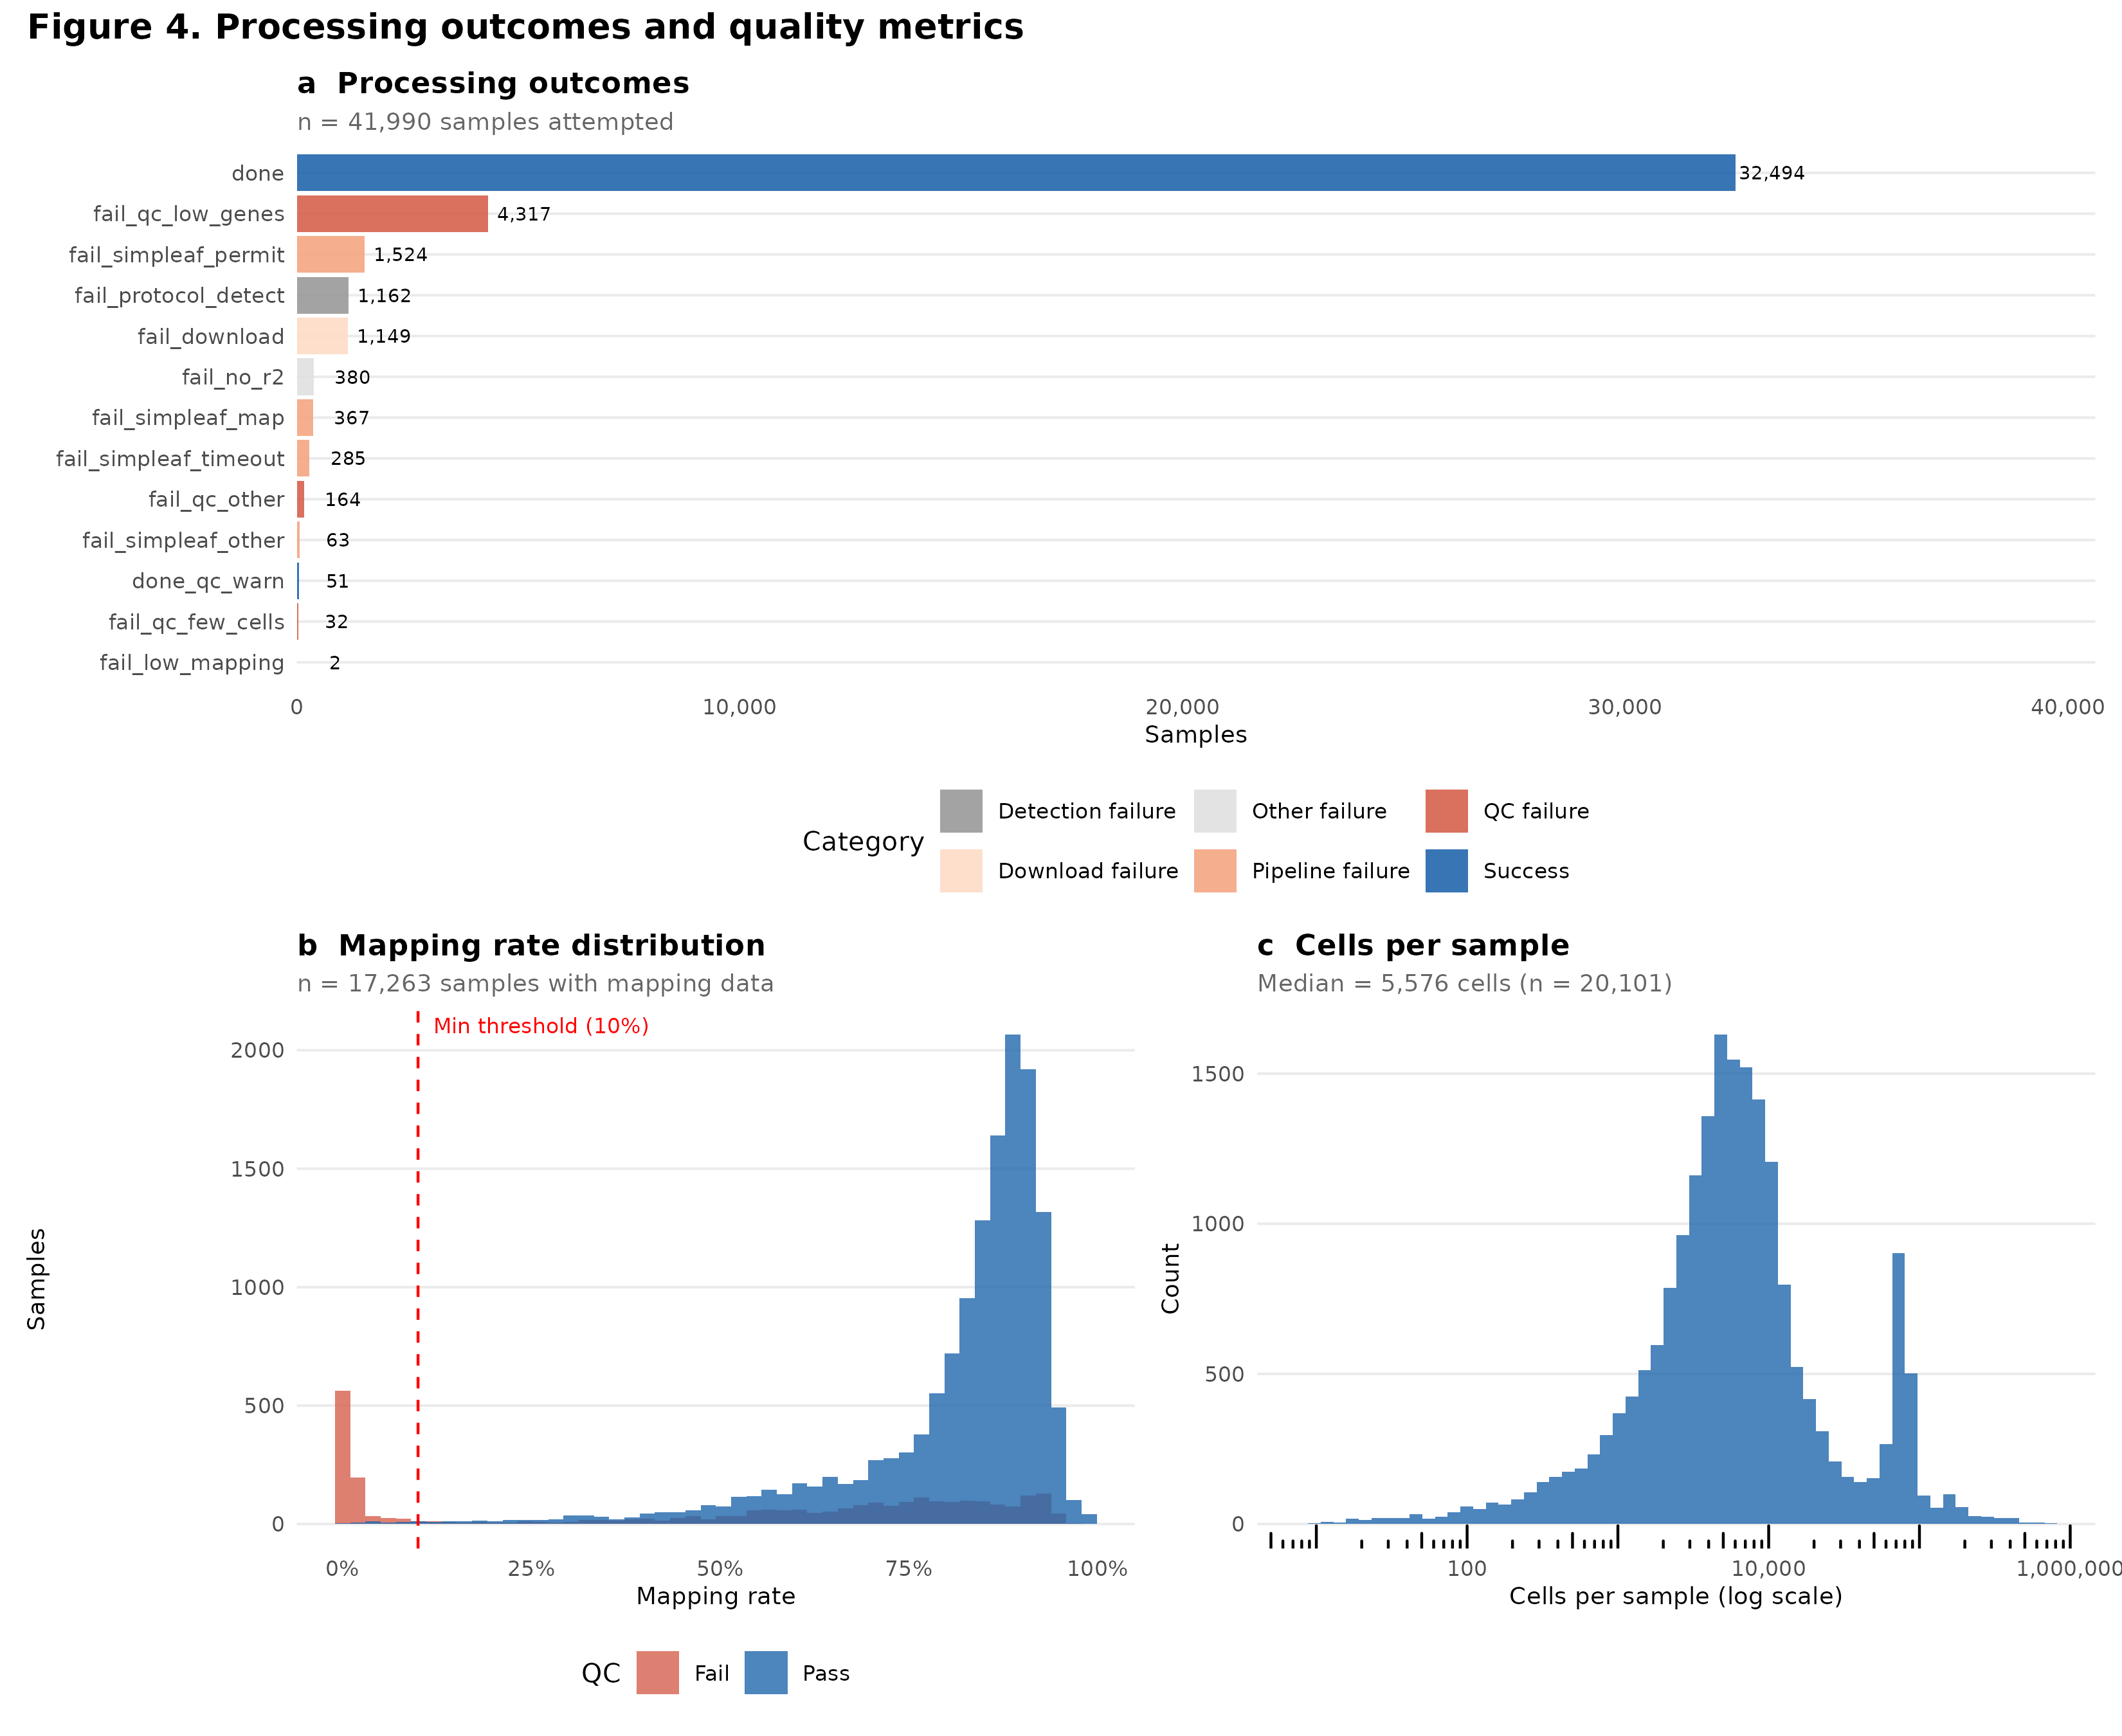
\includegraphics[width=\textwidth]{fig4_processing_qc.pdf}
  \caption{\textbf{Processing outcomes and quality metrics.}
    \textbf{(a)}~Distribution of processing status codes for all samples
    that have been submitted to the pipeline. Success (``done'') is the
    most common outcome; permit-list failures and protocol detection
    failures are the dominant failure modes.
    \textbf{(b)}~Distribution of mapping rates across processed samples.
    The dashed red line indicates the 10\% minimum threshold.
    \textbf{(c)}~Distribution of cells per sample (log scale) for samples
    with cell count data.}
  \label{fig:qc}
\end{figure*}

\begin{figure*}[t]
  \centering
  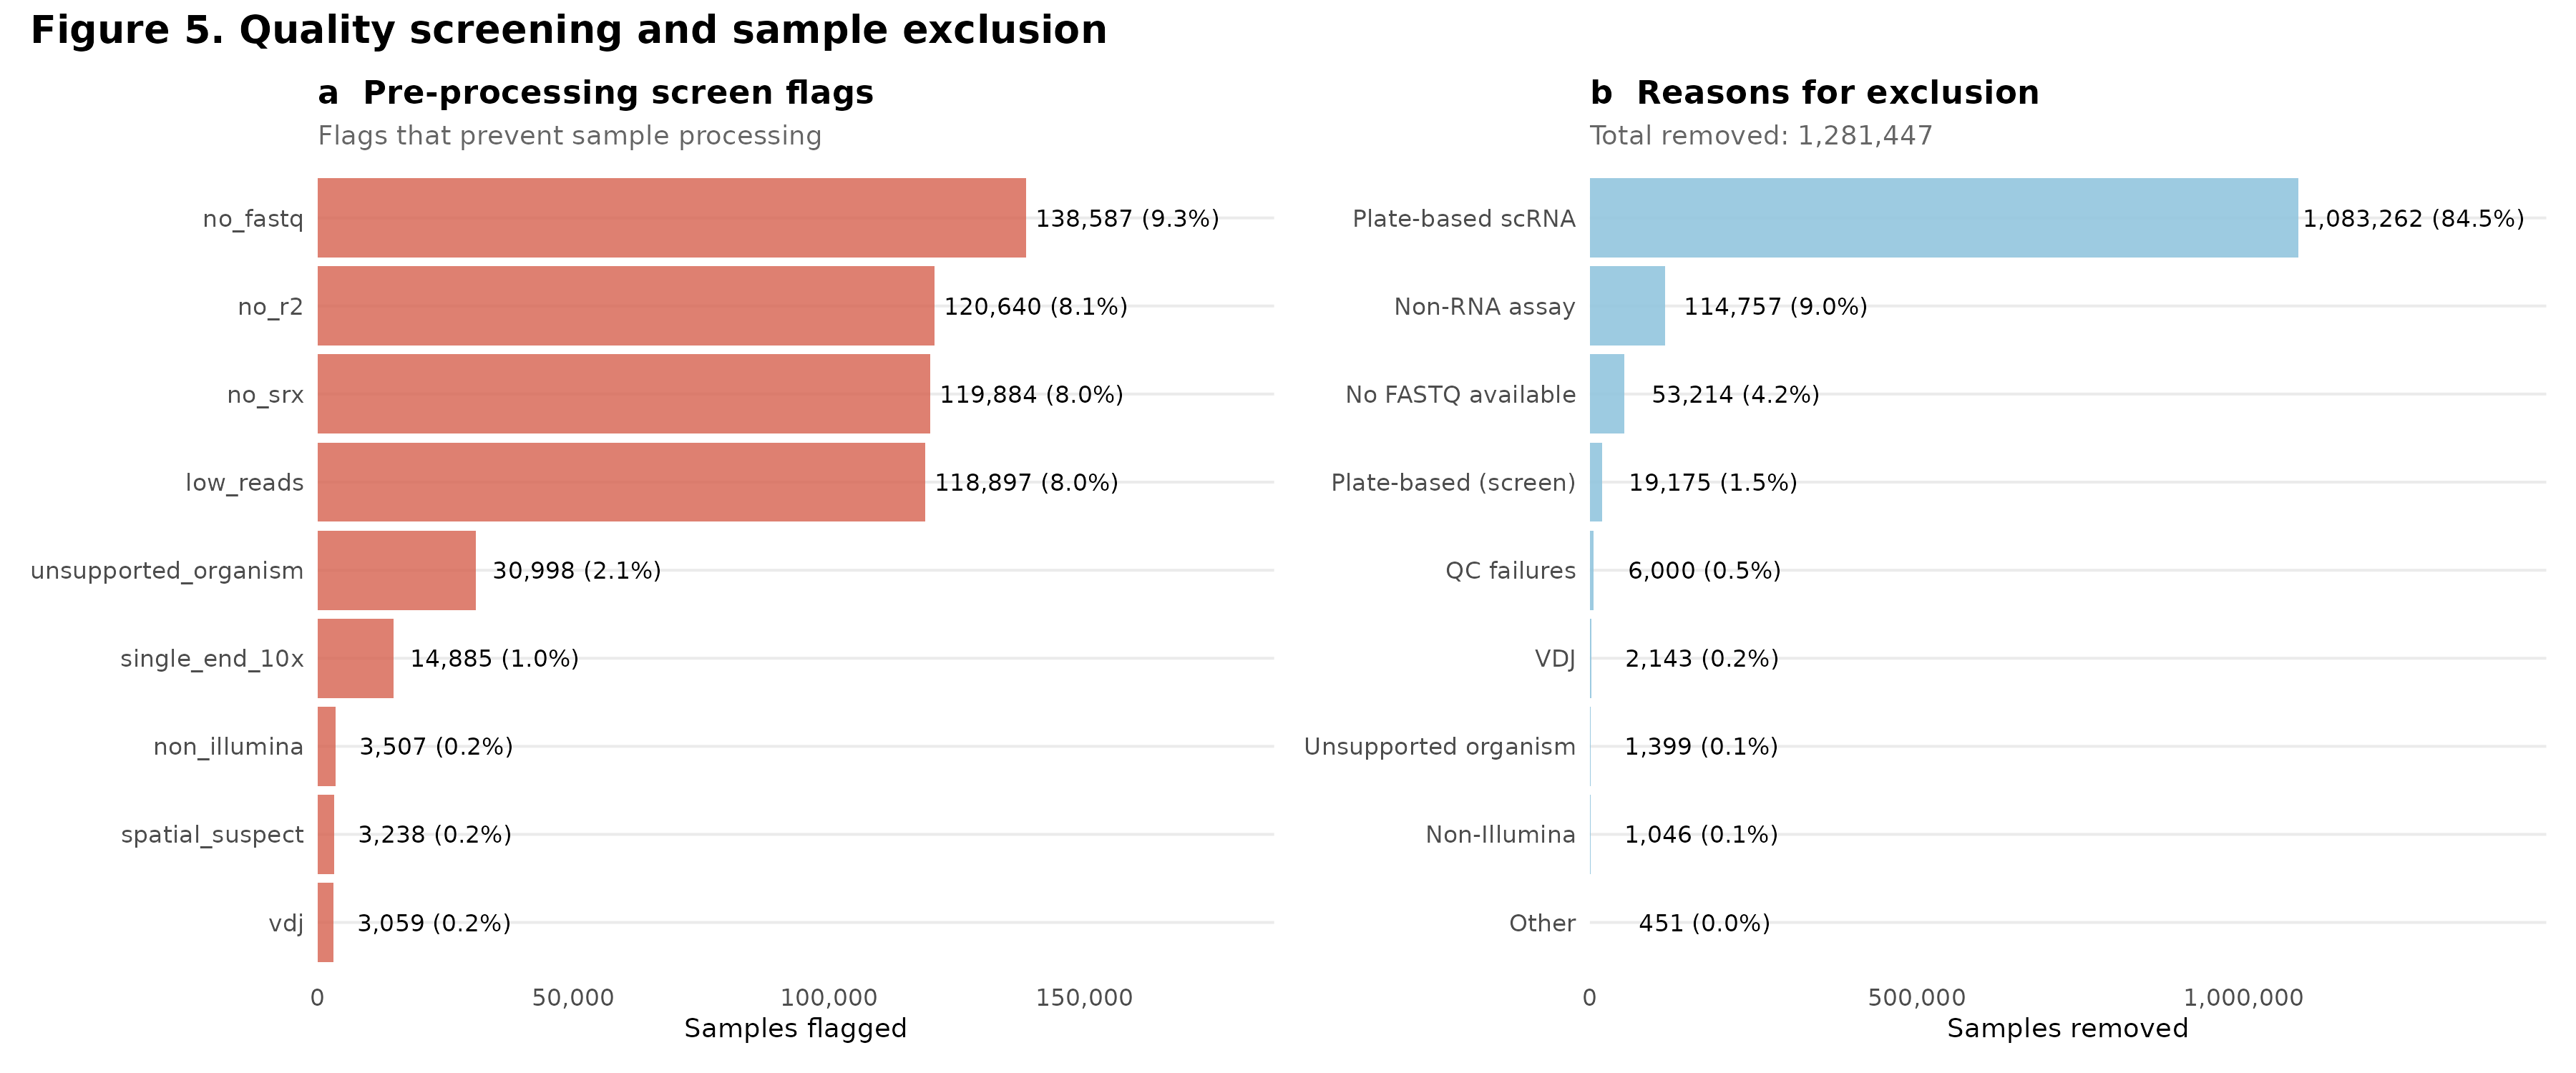
\includegraphics[width=\textwidth]{fig5_screening.pdf}
  \caption{\textbf{Quality screening and sample exclusion.}
    \textbf{(a)}~Pre-processing screen flags applied to the full catalog.
    The most common flags are missing FASTQ files (9.3\%), low read count
    (8.0\%), and missing R2 reads (8.1\%).
    \textbf{(b)}~Breakdown of reasons for excluding 1,281,447 samples
    from processing. Plate-based scRNA-seq (84.5\%) and non-RNA assays
    (9.0\%) account for the vast majority of exclusions.}
  \label{fig:screening}
\end{figure*}

\begin{figure}[t]
  \centering
  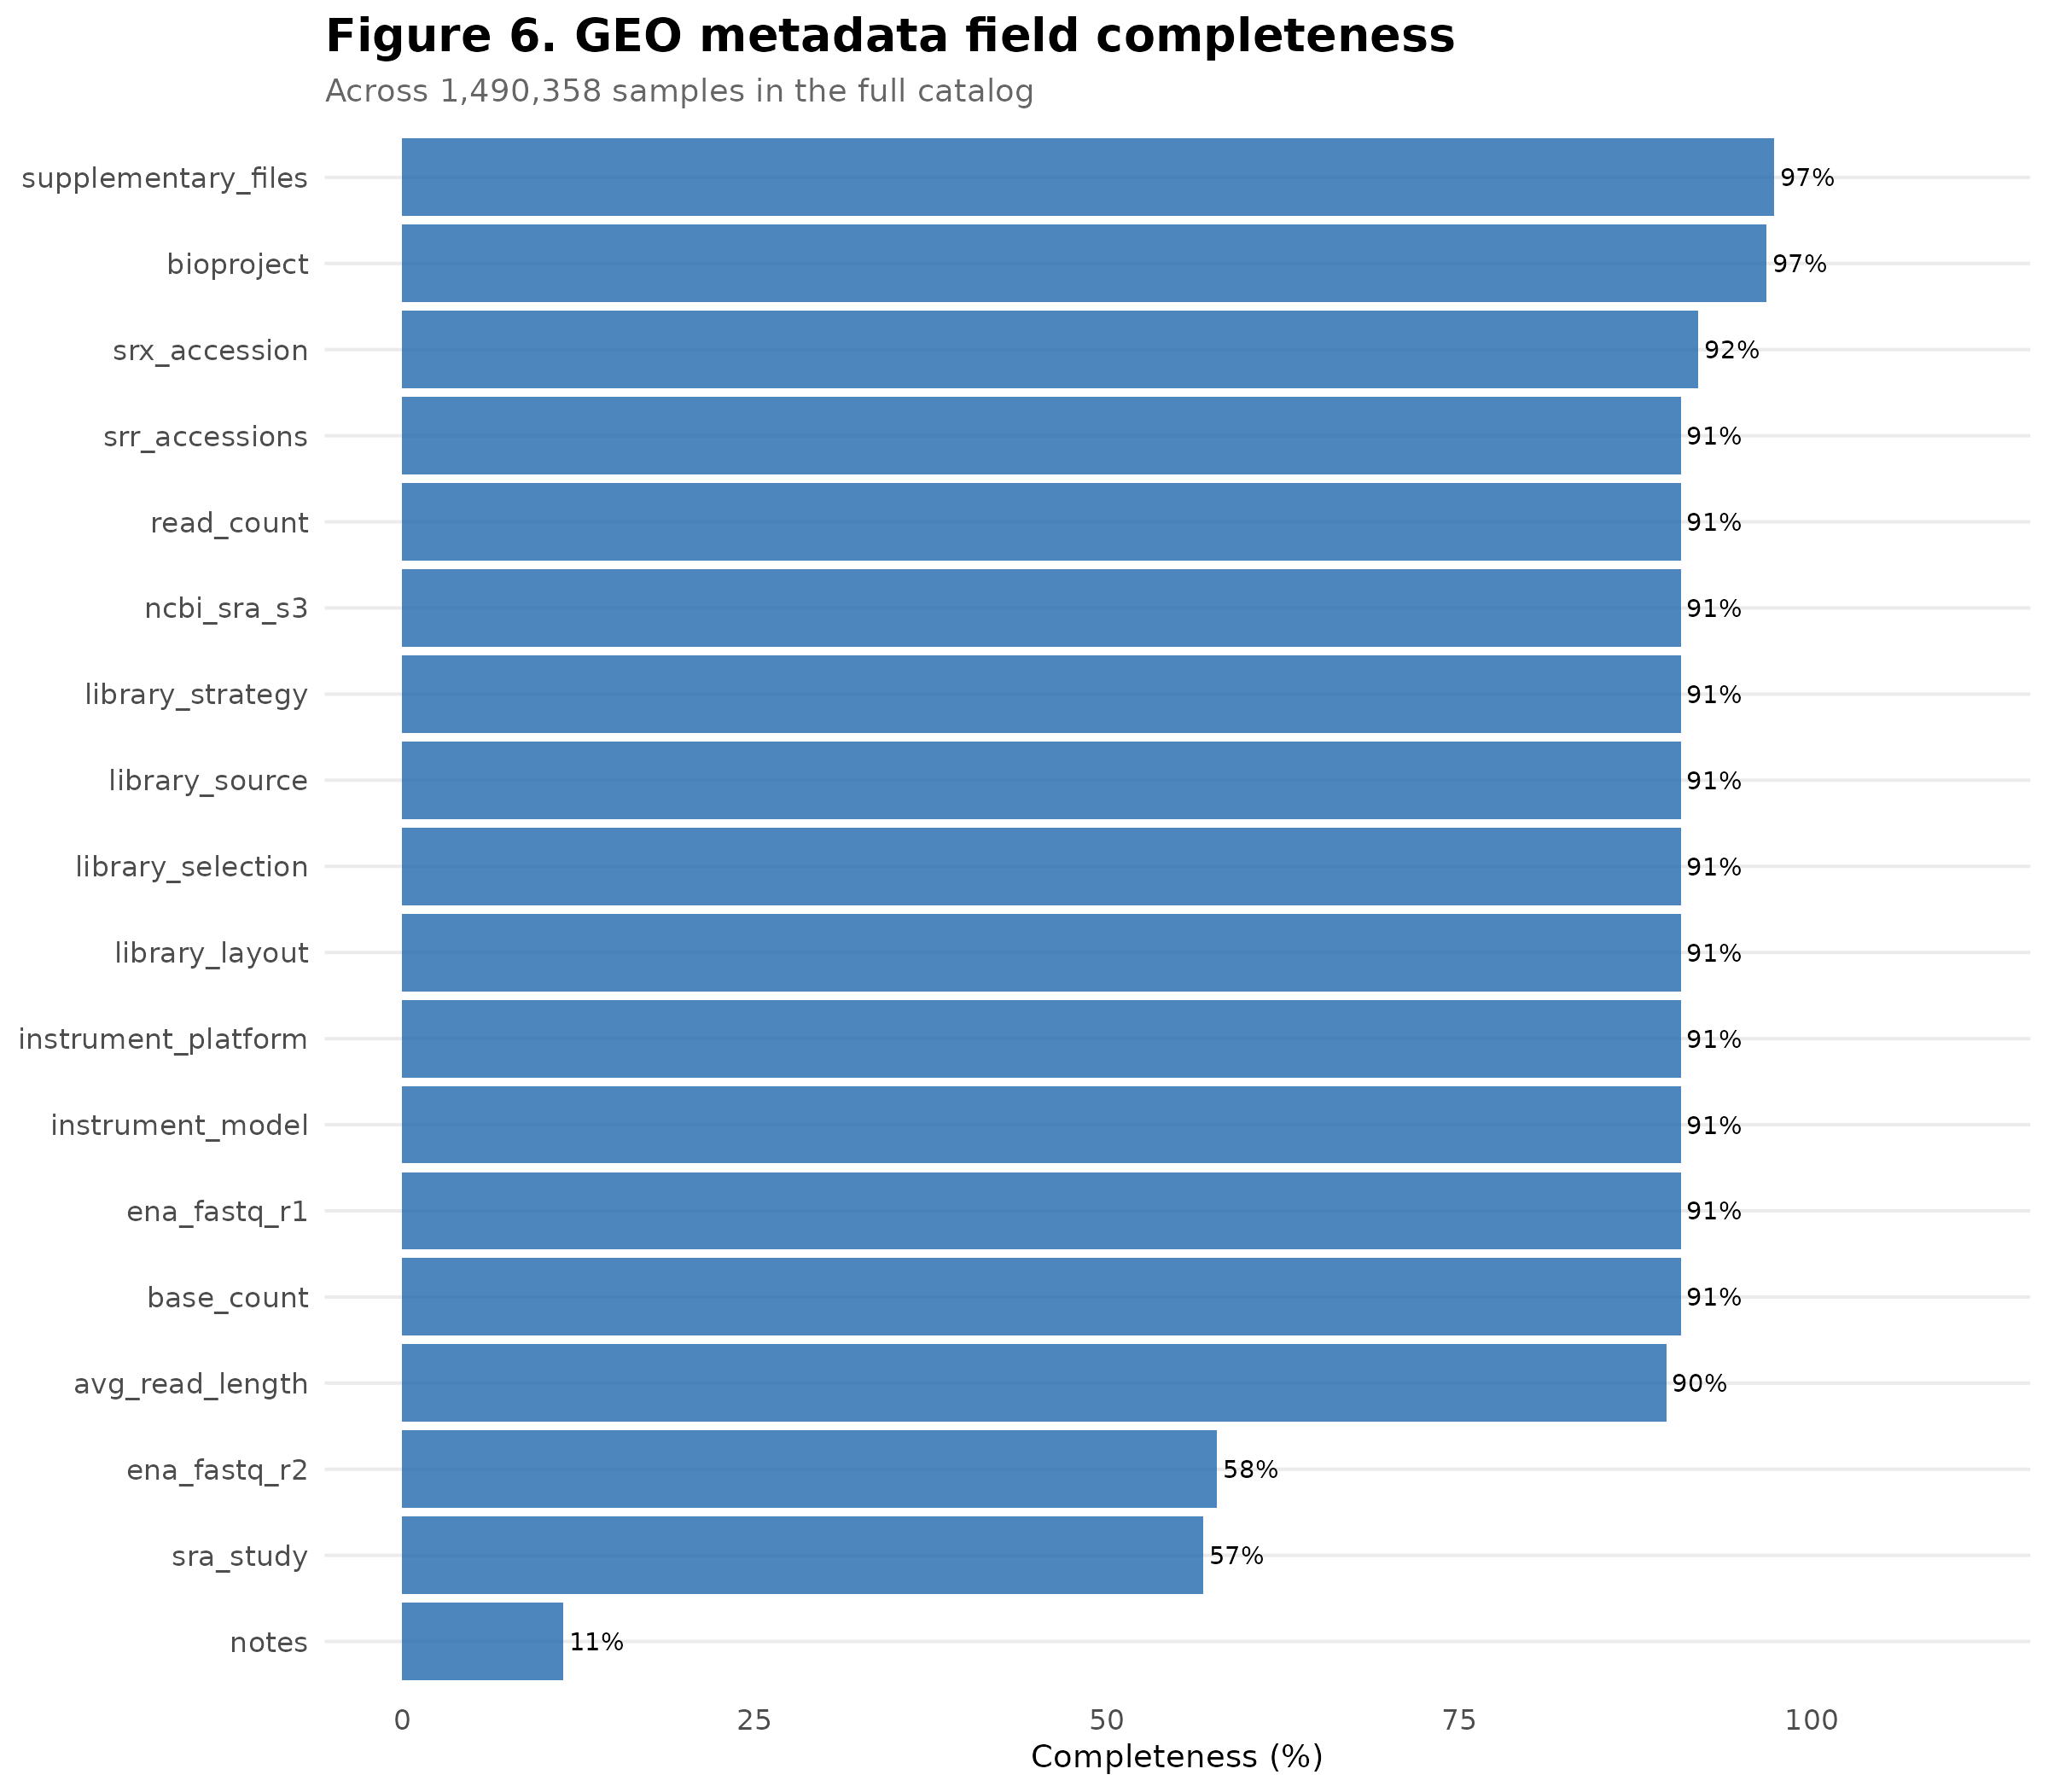
\includegraphics[width=\columnwidth]{fig6_metadata.pdf}
  \caption{\textbf{GEO metadata field completeness.} Percentage of
    non-null, non-empty values for each GEO-derived metadata field across
    all 1,490,358 samples. Core identifiers (GSE, GSM, SRX) and
    biological metadata (organism, summary) are 100\% complete; SRA-derived
    fields (read count, instrument model) are 91\% complete due to samples
    lacking SRA linkage.}
  \label{fig:metadata}
\end{figure}

% ══════════════════════════════════════════════════════════════════
% TABLES
% ══════════════════════════════════════════════════════════════════

\begin{table}[t]
  \centering
  \caption{\textbf{singletDB catalog summary statistics.}}
  \label{tab:catalog}
  \small
  \begin{tabular}{lr}
    \toprule
    \textbf{Metric} & \textbf{Value} \\
    \midrule
    Total GEO samples cataloged & 1,490,358 \\
    Unique GEO series (GSE) & 22,601 \\
    Processable samples & 208,911 (14.0\%) \\
    Processable series & 12,112 \\
    Processing attempted & $\sim$40,000 \\
    QC-passing samples & 32,545 \\
    Total cells quantified & $\sim$1.95 billion \\
    Unique organisms in catalog & 499 \\
    Supported species (with index) & 57 \\
    Matched organisms & 268 (99.5\% of samples) \\
    Sequencing chemistries supported & 24 \\
    Catalog metadata fields & 70 \\
    \bottomrule
  \end{tabular}
\end{table}

\begin{table}[t]
  \centering
  \caption{\textbf{Supported sequencing chemistries.} Each protocol maps to
    an FGDL chemistry string specifying barcode (b), UMI (u), skip (x),
    and cDNA (r) positions. All non-10x chemistries use the knee-distance
    method for permit-list generation.}
  \label{tab:protocols}
  \small
  \begin{tabular}{llr}
    \toprule
    \textbf{Protocol} & \textbf{Chemistry} & \textbf{Samples} \\
    \midrule
    10x Chromium v3   & \texttt{10xv3} (builtin) & 48,402 \\
    10x Chromium v2   & \texttt{10xv2} (builtin) & 11,464 \\
    10x 5$'$ v3       & \texttt{10xv3}  & 9,265 \\
    10x Chromium v4   & \texttt{10xv4-3p} (builtin) & 361 \\
    10x Multiome      & \texttt{10xv3}  & 2,440 \\
    Drop-seq          & \texttt{1\{b[12]u[8]x:\}} & 2,494 \\
    inDrop            & \texttt{1\{b[8]x[22]b[8]u[6]\}} & 27,365 \\
    BD Rhapsody       & \texttt{1\{b[9]x[12]b[9]x[13]b[9]u[8]\}} & 1,388 \\
    sci-RNA-seq3      & \texttt{1\{b[10]x[6]u[8]b[10]\}} & 14,394 \\
    SPLiT-seq         & \texttt{1\{r:\}2\{u[10]b[8]x[30]...\}} & --- \\
    Parse Biosciences & \texttt{1\{r:\}2\{u[10]b[8]x[30]...\}} & 1,046 \\
    DNBelab           & \texttt{1\{b[10]u[10]x:\}} & 663 \\
    Seq-Well          & \texttt{1\{b[12]u[8]x:\}} & 369 \\
    ddSEQ             & \texttt{1\{u[8]b[7]x[10]b[7]...\}} & 285 \\
    Microwell-seq     & \texttt{1\{b[18]u[6]x:\}} & --- \\
    \bottomrule
  \end{tabular}
\end{table}

\begin{table}[t]
  \centering
  \caption{\textbf{Quality control thresholds.} Low-sensitivity protocols
    include Drop-seq, Seq-Well, Microwell-seq, SureCell, CEL-seq/2,
    MARS-seq, STRT-seq, iCELL8, Scope-seq, and ddSEQ.}
  \label{tab:qc}
  \small
  \begin{tabular}{lcc}
    \toprule
    \textbf{Parameter} & \textbf{Standard} & \textbf{Low-sensitivity} \\
    \midrule
    Min.\ cells detected & 10 & 10 \\
    Min.\ mapping rate & 10\% & 10\% \\
    Min.\ median genes/cell & 50 & 20 \\
    Min.\ unspliced fraction & 1\% & 1\% \\
    \bottomrule
  \end{tabular}
\end{table}

\begin{table}[t]
  \centering
  \caption{\textbf{Comparison with existing single-cell data resources.}}
  \label{tab:comparison}
  \small
  \begin{tabularx}{\columnwidth}{lXXXX}
    \toprule
    & \textbf{singletDB} & \textbf{CELLxGENE} & \textbf{DISCO} & \textbf{PanglaoDB} \\
    \midrule
    Source & GEO FASTQ & Published mtx & Published mtx & GEO FASTQ \\
    Reprocessing & Uniform & No & No & Uniform \\
    Aligner & piscem & N/A & N/A & HISAT2 \\
    Species & 57 & Human, mouse & Human, mouse & Human, mouse \\
    Chemistries & 24 & N/A & N/A & 3 \\
    USA counts & Yes & No & No & No \\
    Cell types & Planned & Yes & Yes & Yes \\
    Active & Yes & Periodic & Periodic & No (2020) \\
    Cells & $\sim$1.95B & $>$100M & $\sim$18M & $\sim$5.7M \\
    \bottomrule
  \end{tabularx}
\end{table}

\begin{table}[t]
  \centering
  \caption{\textbf{Pipeline software and parameters.}}
  \label{tab:software}
  \small
  \begin{tabular}{ll}
    \toprule
    \textbf{Component} & \textbf{Version / Parameter} \\
    \midrule
    simpleaf & 0.19.5 \\
    piscem (mapper) & 0.14.6 ($k = 31$, $m = 19$) \\
    alevin-fry & 0.11.2 \\
    Quantification mode & USA (unspliced/spliced/ambiguous) \\
    UMI resolution & \texttt{cr-like} \\
    Splici index \texttt{rlen} & 91 \\
    Reference genomes & Ensembl 111--113 / Genomes 59 \\
    Gene annotation & GENCODE v45/vM34; Ensembl 111--113 \\
    Permit-list (10x) & Unfiltered manufacturer whitelist \\
    Permit-list (other) & Knee $\to$ expect-5000 $\to$ expect-500 \\
    Output format & VOCSC + Zstandard L3 (\texttt{.1pz}) \\
    Kraken2 database & PlusPF (confidence = 0.2) \\
    \bottomrule
  \end{tabular}
\end{table}

% ══════════════════════════════════════════════════════════════════
% REFERENCES
% ══════════════════════════════════════════════════════════════════

\bibliography{refs}

\end{document}
